\documentclass[../../../include/open-logic-section]{subfiles}

\begin{document}

\olfileid{sth}{ordinals}{idea}
\olsection{序数的一般概念}

考虑按通常顺序排列的自然数：

\begin{center}
	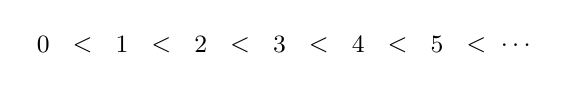
\begin{tikzpicture}
	\foreach \x/\xtext in {0, 1, 2, 3, 4, 5}
	{
		\node (\x a) at (\x, 1) {\small{$\x$}};
		\node (\x a) at (\x.5, 1) {\small{$<$}};
	}
	\node (ldots) at (6, 1) {\small{$\ldots$}};
	\end{tikzpicture}
\end{center}

用术语来说，我们称之为一个$\omega$-序列。的确，这种一般的序体现在我们最初构造集合层级各阶段的方式中。但现在设想我们将$0$移到此序列的末尾，使其排在所有其他数之后：

\begin{center}
	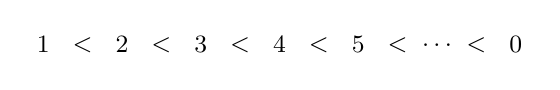
\begin{tikzpicture}
	\foreach \x/\xtext in {1, 2, 3, 4, 5}
	{
		\node (\x a) at (\x, 1) {\small{$\x$}};
		\node (\x a) at (\x.5, 1) {\small{$<$}};
	}
	\node (ldots) at (6, 1) {\small{$\ldots$}};
	\node (bea) at (6.5, 1) {\small{$<$}};
	\node (noa) at (7, 1) {\small{$0$}};
	\end{tikzpicture}
\end{center}

这里的实体相同，但排序方式有着根本的不同：我们第一个序没有最后元素；而新序有。事实上，我们的新序由一个$\omega$-序列的实体（$1, 2, 3, 4, 5, \ldots$）后接另一个实体构成。这便是一个$\omega+1$-序列。

仅用这些实体，我们还能生成更多类型的序。例如，考虑所有偶数（按自然顺序）后接所有奇数（按自然顺序）：

\begin{center}
	\begin{tikzpicture}
	\node(a1) at (1,1) {\small{$0$}};
	\node(a2) at (1.5,1) {\small{$<$}};
	\node(a3) at (2,1) {\small{$2$}};
	\node(a4) at (2.5,1) {\small{$<$}};
	\node(a5) at (3,1) {\small{$4$}};
	\node(a6) at (3.5,1) {\small{$<$}};
	\node(dots) at (4,1) {\small{$\ldots$}};
	\node(aaoe) at (4.5,1) {\small{$<$}};
	\node(b1) at (5,1) {\small{$1$}};
	\node(b2) at (5.5,1) {\small{$<$}};
	\node(b3) at (6,1) {\small{$3$}};
	\node(b4) at (6.5,1) {\small{$<$}};
	\node(b5) at (7,1) {\small{$\ldots$}};
	\end{tikzpicture}
\end{center}

这是一个$\omega$-序列后接另一个$\omega$-序列；即一个$\omega+\omega$-序列。

当然，我们可以继续下去。但我们想要的是一种一般性的方法，来理解关于\emph{序}的这些说法。

\end{document}